\subsection{APPROXIMATION OF CONTINUOUS MAPPINGS OF A COMPACT SPACE INTO A NORMED SPACE}

Let X be a compact space and let Y be a normed vector space over the field R (Chapter IX, § 3); the space \(\mathcal{C}(\mathbf{X};\mathbf{Y})\) will always be assumed to carry the topology of uniform convergence defined by the norm \(||u|| = \sup_{x\in \mathbf{X}}||u(x)||\) (§ 3, no. 2).

Given a set \(\mathbf{H}\) of continuous real-valued functions defined on \(\mathbf{X}\) , a finite family \((u_i)_{1\leqslant i\leqslant n}\) of functions belonging to \(\mathbf{H}\) , and a finite family \((a_i)_{1\leqslant i\leqslant n}\) of points of \(\mathbf{Y}\) : the mapping \(x\to \sum_{i = 1}^{n}a_iu_i(x)\) of \(\mathbf{X}\) into \(\mathbf{Y}\) is then continuous; we denote it by \(\sum_{i = 1}^{n}a_iu_i\) , and we say that it is a linear combination of functions of \(\mathbf{H}\) with coefficients in \(\mathbf{Y}\) . We say that a continuous mapping \(f:\mathbf{X}\rightarrow \mathbf{Y}\) can be uniformly approximated by linear combinations of functions of \(\mathbf{H}\) (with coefficients in \(\mathbf{Y}\) ), if \(f\) lies in the closure of the vector subspace of \(\mathcal{C}(\mathbf{X};\mathbf{Y})\) formed by these linear combinations.

PROPOSITION 5. Let X be a compact space, Y a normed space over R and H a subset of C (X; R). If every continuous real-valued function on X can be uniformly approximated by functions of H, then every continuous mapping f of X into Y can be uniformly approximated by linear combinations of functions of H with coefficients in Y.

Given any real number \(\varepsilon > 0\) , for each \(x \in \mathbf{X}\) there exists an open neighbourhood of \(x\) in which the oscillation of \(f\) is \(\leqslant \varepsilon\) . Hence there is a finite open covering \((\mathrm{A}_i)_{1 \leqslant i \leqslant n}\) of \(\mathbf{X}\) such that the oscillation of \(f\) in each \(\mathrm{A}_i\) is \(\leqslant \varepsilon\) . Let \(\boldsymbol{a}_i\) be a value of \(f\) in \(\mathrm{A}_i\) ( \(1 \leqslant i \leqslant n\) ), and let \((u_i)_{1 \leqslant i \leqslant n}\) be a continuous partition of unity subordinate to the covering \((\mathrm{A}_i)\) (Chapter IX, § 4, no. 4, Corollary to Proposition 4). Let \(x\) be any point of \(\mathbf{X}\) . For each index \(i\) such that \(x \notin \mathrm{A}_i\) , we have \(u_i(x) = 0\) , and for each index \(i\) such that \(x \in \mathrm{A}_i\) we have \(||f(x) - a_i|| \leqslant \varepsilon\) ; it follows that

\[
\left\| \boldsymbol {f} (x) - \sum_ {i = 1} ^ {n} \boldsymbol {a} _ {i} u _ {i} (x) \right\| = \left\| \sum_ {i = 1} ^ {n} (\boldsymbol {f} (x) - \boldsymbol {a} _ {i}) u _ {i} (x) \right\| \leqslant \varepsilon \sum_ {i = 1} ^ {n} u _ {i} (x) = \varepsilon .
\]

On the other hand, by hypothesis there is a function \(v_{i} \in \mathbf{H}\) such that

\[
\left| u _ {i} (x) - v _ {i} (x) \right| \leqslant \frac {\varepsilon}{\sum_ {j = 1} ^ {n} | | \boldsymbol {a} _ {j} | |}
\]

for all \(x \in \mathbf{X} (1 \leqslant i \leqslant n)\) ; hence we have

\[
\left\| \boldsymbol {f} (x) - \sum_ {i = 1} ^ {n} \boldsymbol {a} _ {i} v _ {i} (x) \right\| \leqslant 2 \varepsilon \text {   for   all   } x \in \mathbf {X},
\]

and the proof is complete.

From Proposition 5 it follows that, to each of the propositions in which we have proved that a certain subset H of C(X; R) is dense, there corresponds an analogous proposition for continuous mappings of X into an arbitrary normed space Y. We shall write down explicitly only the proposition which corresponds in this way to Theorem 3. Given a set H of real-valued functions on X, a polynomial in the functions of H, with coefficients in Y, is defined to be any linear combination, with coefficients in Y, of products of a finite (possibly empty) family of functions belonging to H. Then:

PROPOSITION 6. Let X be a compact space and let H be a set of continuous real-valued functions on X which separates the points of X. Then every continuous mapping of X into a normed space Y over R can be uniformly approximated by polynomials in the functions of H with coefficients in Y.

From this we deduce :

PROPOSITION 7. Let X be a compact space and let H be a set of continuous complex-valued functions on X which separates the points of X. Then every continuous mapping of X into a normed space Y over C can be uniformly approximated by polynomials in the functions \(f \in \mathbf{H}\) and their conjugates \(\overline{f}\) with coefficients in Y.

We have only to note that Y is also a normed space over R and to apply Proposition 6 to the set of real parts and imaginary parts of the functions \(f \in H\) , using the formulas

\[
\mathfrak {R} f = \frac {1}{2} (f + \overline {{f}}), \quad \Im f = \frac {1}{2 i} (f - \overline {{f}}).
\]

COROLLARY 1. If X is a compact subset of the space \(\mathbf{C}^n\) , then every continuous mapping \((z_1, z_2, \ldots, z_n) \to f(z_1, z_2, \ldots, z_n)\) of X into a normed space Y over the field C can be uniformly approximated by polynomials in the \(z_k\) and \(\overline{z}_k\) with coefficients in Y.

\pandocbounded{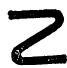
\includegraphics[keepaspectratio]{images/part002_94458643.jpg}}

We shall see later that in general it is not possible to approximate f uniformly by polynomials (with coefficients in Y) in the variables \(z_{k}\) alone, even if Y = C.

COROLLARY 2. Let X be a locally compact space and let \(\mathcal{C}_0(\mathbf{X})\) be the normed C-algebra of continuous mappings of X into C which tend to 0 at infinity. Let A be a subalgebra of \(\mathcal{C}_0(\mathbf{X})\) which separates the points of X and is such that (i) \(\overline{f} \in \mathbf{A}\) whenever \(f \in \mathbf{A}\) , (ii) for each \(x \in \mathbf{X}\) , there is an \(f \in \mathbf{A}\) such that \(f(x) \neq 0\) . Then A is dense in \(\mathcal{C}_0(\mathbf{X})\) .

If \(X'\) is the compact space obtained by adjoining a point at infinity \(\omega\) to X, then \(\mathcal{C}_{0}(\mathbf{X})\) can be identified with the subspace of \(\mathcal{C}(\mathbf{X};\mathbf{C})\) consisting of continuous mappings which vanish at \(\omega\) , the norm on \(\mathcal{C}_{0}(\mathbf{X})\) being defined by

\[
\left| \left| f \right| \right| = \sup _ {x \in \mathbf {X}} | f (x) | = \sup _ {x \in \mathbf {X}'} | f (x) |.
\]

By virtue of Proposition 7, every \(f \in \mathcal{C}_{0}(X)\) can be uniformly approximated by polynomials with complex coefficients in the functions belonging to A; moreover, since \(f(\omega) = 0\) , the argument of no. 2, Proposition 4 shows that we may suppose these polynomials to have no constant term, and then they belong to A.

Another application of Proposition 7 is the following :

PROPOSITION 8. Let P be the set of all periodic continuous mappings of \(\mathbf{R}^m\) into \(\mathbf{C}\) whose group of periods contains \(\mathbf{Z}^m\) . Then every function belonging to P can be uniformly approximated in \(\mathbf{R}^m\) by linear combinations, with complex coefficients, of functions of the form

\[
(x _ {1}, x _ {2}, \dots , x _ {m}) \rightarrow e (h _ {1} x _ {1} + h _ {2} x _ {2} + \dots + h _ {m} x _ {m}),
\]

where the \(h_{i}\) are rational integers (such linear combinations are called trigonometric polynomials in m variables).

We have only to observe that P (endowed with the topology of uniform convergence) is canonically isomorphic to the space of all continuous mappings of the compact space \(T^{m}\) into C (Chapter VII, § 1, no. 6), and apply Proposition 7 to the set of mappings of \(T^{m}\) into C which correspond to the m mappings \((x_{1}, x_{2}, \ldots, x_{m}) \to e(x_{i}) \quad (1 \leqslant i \leqslant m)\) of \(R^{m}\) into C.

\ExerciseGroupsStart

